\documentclass[letterpaper, 10 pt, conference]{ieeeconf}  % Comment this line out if you need a4paper
%\documentclass[a4paper, 10pt, conference]{ieeeconf}      % Use this line for a4 paper
\IEEEoverridecommandlockouts                              % This command is only needed if 
                                                          % you want to use the \thanks command
\overrideIEEEmargins                                      % Needed to meet printer requirements.

\usepackage[english]{babel}
\usepackage[utf8]{inputenc}

% The preceding line is only needed to identify funding in the first footnote. If that is unneeded, please comment it out.
\usepackage{cite}
\usepackage{amsmath,amssymb,amsfonts}
\usepackage{algorithm}
\usepackage{algpseudocodex}
\usepackage{graphicx}
\usepackage{textcomp}
\usepackage{xcolor}
\usepackage{multicol}
\usepackage{multirow}
\usepackage[export]{adjustbox}
% \usepackage{movie15}


% \usepackage{subcaption}
% \usepackage{caption}
\newcommand{\Madhav}[1]{{\color{magenta}{\textbf{MK}: #1}}}
\newcommand{\Vineet}[1]{{\color{blue}{\textbf{VG}: #1}}}
\def\etal{\textit{et al.}}

\begin{document}

\title{\LARGE \bf Language Guided Navigation in Dynamic Environment\\
%{\footnotesize \textsuperscript{*}Note: Sub-titles are not captured in Xplore and
%should not be used}
% \thanks{\textsuperscript{1} KCIS, International Institute of Information Technology, Hyderabad}
% \thanks{\textsuperscript{*} Equal contribution from the first three authors.}
}

\author{{Author 1 }
\and
{ Author 2 }
%\IEEEauthorblockA{\textit{dept. name of organization (of Aff.)}}
\and
{ Author 3 }
%\IEEEauthorblockA{\textit{dept. name of organization (of Aff.)}}
\and
{Author 4 }
%\IEEEauthorblockA{\textit{dept. name of organization (of Aff.)}}
\and
{ Author 5} 
\and
{ Author 6} 
\and
{ Author 7} 
%\IEEEauthorblockA{\textit{dept. name of organization (of Aff.)}}
%{ KCIS, International Institute of Information Technology, Hyderabad }
} 

%%%%% TODO %%%%%
% 1. Interpretable Trajectory Prediction
% 2. Meta Dataset 
% 3. Explainability
% 4. Give Name to Dataset

\maketitle

\begin{abstract}
Navigation in the dynamically changing real world is a challenging task, and conditioning it on linguistic commands makes it an even more challenging problem. Humans effortlessly perform language-guided navigation in their daily lives, and with this work, we take a step towards imparting autonomous vehicles with similar capabilities. In order to perform language-guided navigation in the dynamic world, we need to simultaneously reason about the linguistic command and the dynamic visual world, both temporally and spatially. To this end, we propose a novel language grounding model that localizes the goal region corresponding to the language command and provides interpretable intermediate trajectory predictions to navigate towards the goal region. Additionally, we release a novel video-language navigation meta-dataset in the Carla environment. We provide extensive quantitative and qualitative empirical results to validate the effectiveness of our approach. Finally, we perform real-time efficacy of the proposed approach.

\end{abstract}

\section{Introduction}

% Introduction to the problem
Humans have exceptional navigational abilities, which, combined with their visual and linguistic prowess, allow them to perform navigation based on the linguistic description of the objects of interest in the environment. This is in direct consequence with the human capability of associating visual objects with their linguistic descriptions. The task of visual grounding is concerned with localizing objects or regions in an image based on a natural language query. Visual grounding is a critical part of language-guided navigation as the first step involves comprehending the linguistic instruction and then performing localization based on it. In autonomous navigation, this problem is formally known as Referring Navigable Regions (RNR)~\cite{rufus2021grounding}, and the goal is to ground navigable regions in an image based on the linguistic command. In this work, we extend the task of RNR to perform language grounding over a dynamically changing scene; additionally, we predict interpretable intermediate trajectories to reach the final destination region referred by the linguistic command.

% Motivation behind the problem
It is commonplace for humans to utilize fine-grained linguistic instructions for executing navigational maneuvers in real-time. Consider the scenario of a passenger in a taxi; the passenger instructs, "turn right from the intersection and stop near the bus stand." The taxi driver must make simultaneous temporal and spatial decisions by asking `When?' and  `Where?'. He has to make real-time decisions regarding `when' to turn right and stop, and `where' to stop. From the RNR perspective, it requires identifying the navigable regions on the road for ``turning right" and a region near the bus stand for ``stopping." Now, suppose the distance between the `bus stand' and the current location is considerable; this scenario becomes particularly challenging as it requires the taxi to keep moving until a `bus stand" becomes visible and then `stop" at a region near it. Our novel dataset consists of multiple such scenarios, which require strong temporal reasoning to successfully navigate to the desired location.

\begin{figure}[t]
    \centering
    \begin{tabular}[t]{p{0.48\textwidth} }
    { \centering \small {\textit{\textbf{Command: }``Stop for the traffic light and then take right and park near the bus stand.''}}}\\
        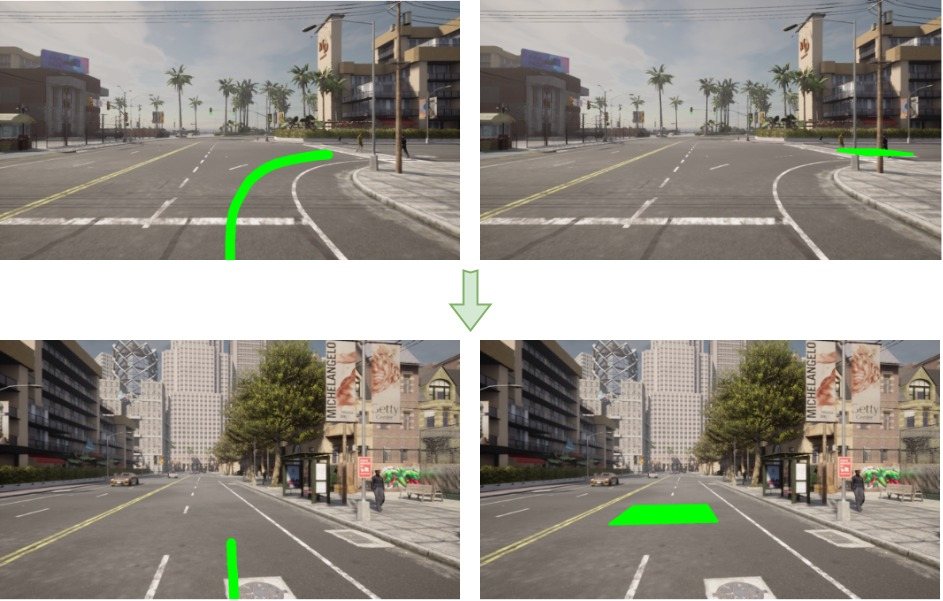
\includegraphics[width=0.48\textwidth]{images/teaser.jpg} \\
        % \includegraphics[width=0.48\textwidth]{images/teaser2.jpg}\\
        % \includegraphics[width=0.48\textwidth]{images/teaser3.jpg}
    \end{tabular}
    \caption{Replace the teaser figure}
    \label{fig:teaser}
\end{figure}

% Existing Approaches
% While there exists several video-based semantic segmentation datasets in the context of autonomous navigation, none of these datasets capture the data that directly influence the task of navigation. For example, a network trained on these semantic segmentation dataset will have knowledge about the semantics of different objects/regions in the environment like road, vehicles, buildings, traffic lights etc; 

While several reinforcement learning-based approaches for language-based navigation exist, they incorporate discrete actions in their Markov decision process formulation. This setting is limited and impractical in realistic scenarios where actions form a continuous space rather than a discrete one. We adopt a visual grounding-based approach to explicitly specify the navigable regions on the road corresponding to the linguistic command.\cite{rufus2021grounding} take a similar approach, but their work only considers image-language pairs for the navigational purpose, and they do not explicitly show live navigation towards the goal region. Instead, we utilize dynamic scenes through video-language pairs to continuously ground the navigable region on the road corresponding to the language command. Additionally, the intermediate trajectory predictions guide the navigation towards the goal region. The entire approach is end-end trainable and promises a new paradigm shift in language-based navigation literature, which is more focused on the visual grounding aspect.

% Our Approach & Contributions
To this end, we propose a novel multi-task network for navigable region prediction and trajectory prediction in a dynamic scene. We explicitly distinguish between intermediate regions and final goal regions for navigable region prediction. The predicted trajectory is interpretable and used to navigate towards the predicted final goal region. Additionally, we propose a novel video-language Navigation meta-dataset in the Carla environment. The proposed dataset is the first of its kind, and it consists of video-language pairs with frame-level annotations. We benchmark the dataset with our novel multi-task network and provide extensive quantitative and qualitative ablation to validate our approach. Finally, we showcase the viability of the proposed approach by performing real-time inference in the Carla environment and successfully executing the language command by navigating to the final goal region based on the trajectory predictions.

To summarize, the main contributions of this paper are the following:
\begin{itemize}

\item We propose a novel multi-task network for predicting navigable regions and intermediate trajectories in a dynamic scene. The prediction for each task is explainable and interpretable in the form of segmentation masks.
\item We present a novel meta-dataset, CARLA-NAV, for video-language navigation task. The dataset is curated using the open source Carla Simulator.
\item We benchmark the dataset using our novel multi-task network and perform extensive ablation studies.
\item We perform real-time language-based navigation with the proposed multi-task network in the Carla environment. We utilize the network predictions and a local planner to successfully navigate the final goal region.

\end{itemize}


\section{Related Work}

\subsection{Visual Grounding}

Visual grounding aims to help associate the linguistic description of entities with their visual counterparts by localizing them visually. There are two prevalent approaches for visual grounding based on the type of localization used. Proposal-based localization is formally referred to as Referring Expression Comprehension (REC). Most methods in REC follow a propose-then-rank strategy, where the ranking is done using similarity scores \cite{rohrbach2016grounding, hu2016natural, plummer2018conditional, rufus2020cosine} or through attention-based methods \cite{deng2018visual, zhang2018grounding, yang2019dynamic, qiu2020language}. The other approach is to localize the objects by their pixel-level segmentation mask, formally known as Referring Image Segmentation (RIS). In RIS, methods use different strategies to fuse the spatial information of the image with the word-level information of the language query \cite{shi2018key, ye2019cross, huang2020referring, jain2021comprehensive}. However, in the context of autonomous navigation, both REC and RIS are limited because they localize the objects, but the problem of how to navigate towards the object still persists. Recently, \cite{rufus2021grounding} proposed the Referring Navigable Region (RNR) task to localize the navigable regions on the road corresponding to the language commands. However, they showcase results on a static image, and they don't show the actual navigation in a dynamic environment. Instead, we propose to extend the RNR task to dynamic video scenes and perform real-time navigation based on language commands.

\subsection{Language-based Navigation}

The objective of language-guided navigation is to allow humans to have the capability to control and influence the navigation of autonomous agents through language commands. Existing Works have utilized imitation learning \cite{nguyen2019vision, nguyen2019help}, behavior cloning \cite{das2018neural}, sequence-sequence translation \cite{anderson2018vision}, and cross-modal attention \cite{huang2019multi, irshad2021hierarchical, cornia2019perceive} based approaches. Most of the literature has focused on indoor environments; both synthetic \cite{kempka2016vizdoom, kolve2017ai2, wu2018building}, and real \cite{chang2017matterport3d, anderson2018vision}. While there are many papers \cite{mirowski2018learning, chen2019touchdown, chancan2020citylearn} on autonomous navigation in outdoor environments, very few of them \cite{sriram2019talk} perform language-based navigation in an outdoor setting. Specifically, \cite{sriram2019talk} predict local waypoints conditioned on the language command to generate trajectories for navigation, but the language commands used by them have less diversity. In this paper, we use diverse linguistic commands with detailed visual descriptions. Additionally, we propose a paradigm shift towards utilizing RNR-based approaches for language-guided navigation, and the CARLA-NAV meta-dataset proposed in this paper is a step towards achieving this goal. 

\section{Dataset}

% This is a meta-dataset, we release the toolkit which can be further used to extend dataset.
% This dataset is first of it's kind and proposes a paradigm shift

The proposed CARLA-NAV dataset was curated using the open-source Carla Simulator for autonomous driving research. It contains episodic level data, where each episode consists of language commands and the corresponding video from Carla Simulator of navigation towards the final goal region described by the command. Each frame from the video is annotated with a segmentation mask corresponding to the intermediate and final navigable regions. The intermediate masks capture the navigable regions traversed by the vehicle until reaching the final goal region corresponding to the language command. Furthermore, we also record the 3d vehicle position in the Carla environment and the camera intrinsic-extrinsic matrices for each frame. For the trajectory prediction task, we take the 3d vehicle position of the vehicle in the successive frames and project the 3d positions to the front-camera image using the projective transformation. We treat trajectory prediction as a dense prediction task to make it interpretable during navigation. 
\Madhav{Will help if some images are available that explain what is mentioned above}

% Some info about meta-dataset
The dataset includes video sequences captured in 8 different maps, 14 distinct weather conditions, and a diverse range of vehicles and passengers in the environment. The language commands in our dataset contain detailed visual descriptions of the environment and describe a wide range of maneuvers. In some cases, there are multiple maneuvers in a single command. Overall, the training split of the dataset consists of 441 video-language pair sequences, and the validation split consists of 25 sequences. In the next section, we describe the dataset creation process.

\begin{figure*}[t]
\centering
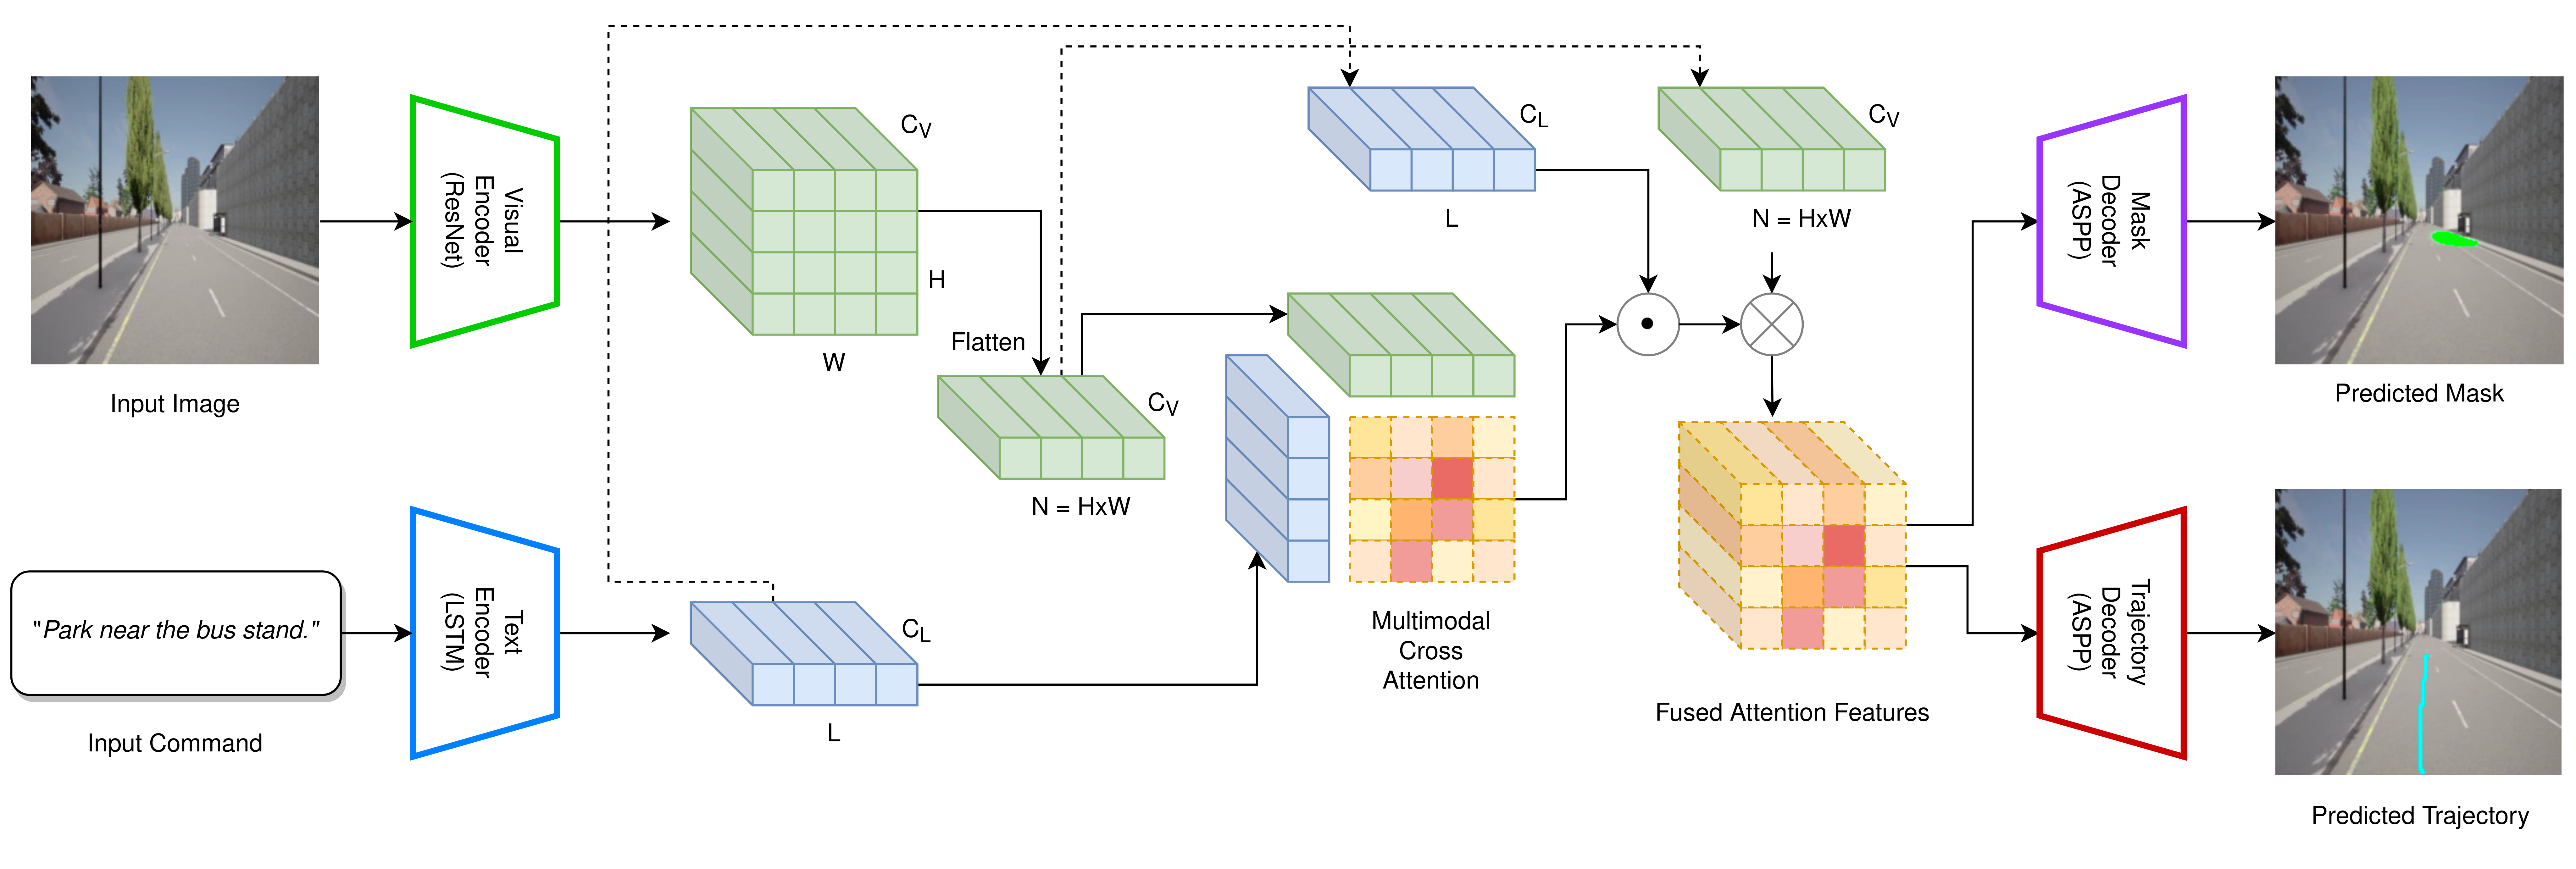
\includegraphics[width=1.0\textwidth]{images/network_arch.png}
\caption{TODO: Add suitable caption to network architecture.}
\label{pipeline}
\end{figure*}

\subsection{Dataset Creation}

% defend rule-based planner? command before or after
We created a data-collection toolkit on top of Carla's API and plan to open-source it upon acceptance. The data collection process can be grouped into two steps: (1) providing a language command that describes the series of navigational maneuvers and (2) navigating the Carla environment based on the language command. Next, we describe each step in detail.
The language commands for navigation were provided manually through a text prompt and were in direct correspondence with the surrounding environment. For navigation, we used mouse clicks to select the navigable regions for the vehicle in the front camera view of the RGB camera and get the 2D point corresponding to the click. We use a depth camera to get the depth corresponding to the 2D pixel and then transform it to the 3D world coordinates using Inverse Projective transform; this 3D position is passed as input to the local planner to navigate the Carla environment. We use a simple rule-based planner for our case; however, this can easily be replaced with more advanced planners like RRT and RRT*. For the trajectory prediction task, we take the 3D vehicle position of the vehicle in the successive frames and project the 3D positions to the front-camera image using the projective transformation. We treat trajectory prediction as a dense prediction task to make it interpretable during navigation. Some language commands contain multiple actionable maneuvers; in this case, we use multiple mouse clicks to guide the navigation. These intermediate mouse clicks signify the intermediate navigable regions, and the last mouse click depicts the final goal region corresponding to the command. We treat the intermediate regions and final regions as two separate classes for segmentation to determine the stopping criterion for the vehicle. Overall, only the language commands and mouse clicks required manual effort, apart from these the data-collection process is fully automated.
Finally, the proposed toolkit can be used to further extend the dataset in multiple ways depending on the use case. 

% \begin{figure*}[t]
% \centering
% 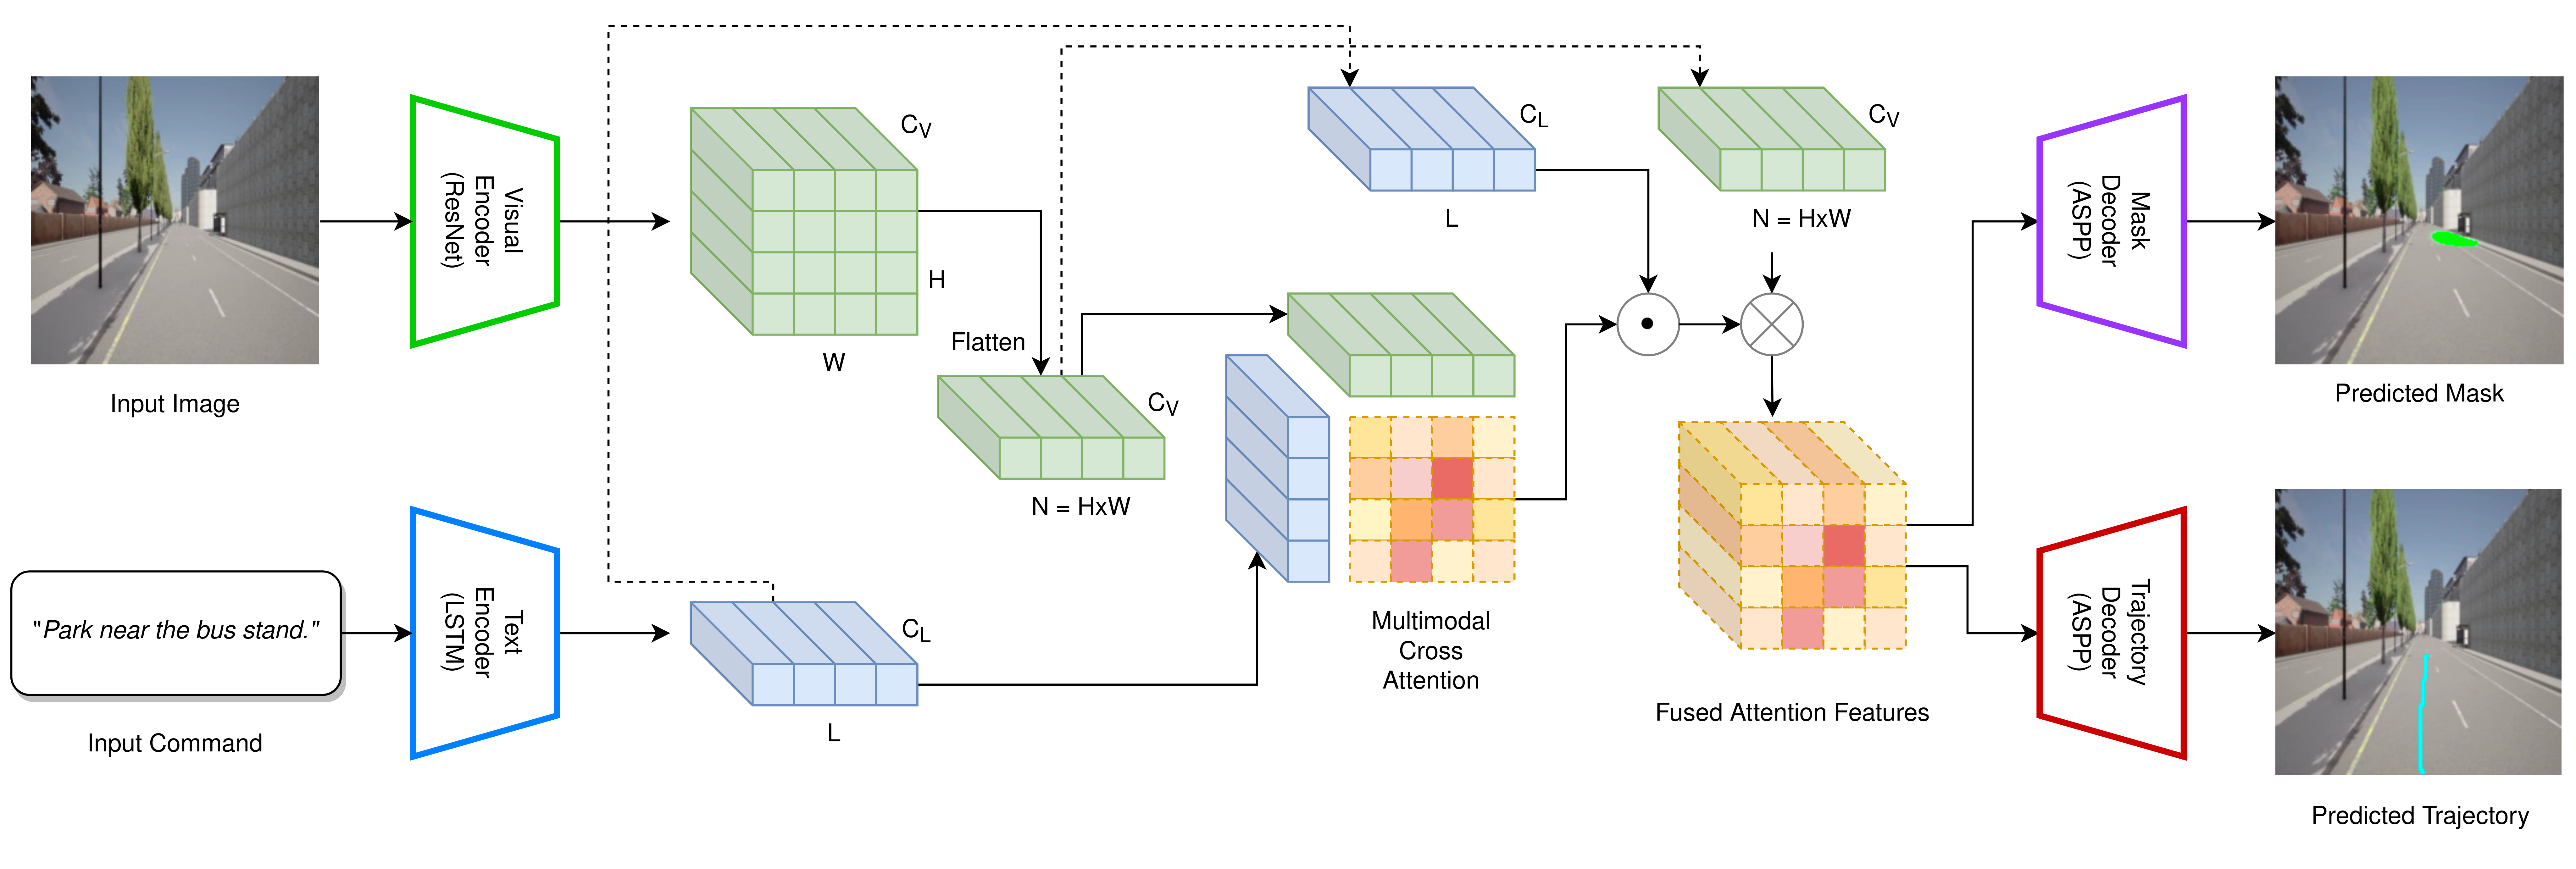
\includegraphics[width=1.0\textwidth]{images/network_arch.png}
% \caption{TODO: Add suitable caption to network architecture.}
% \label{pipeline}
% \end{figure*}

\section{Methodology}

Given a sequence of video frames $V = \{v_1, v_2,..v_T\}$ and a language command $L = \{l_1, l2,..l_N\}$, the goal is to predict the navigable regions $\{y_1, y_2,..y_T\}$ and the trajectory masks $\{z_1, z_2,..z_T\}$ corresponding to each frame. The length of video is represented by $T$ and $N$ represents the maximum number of words in the command. The navigation masks $y_t$ and the trajectory mask $z_t$ for a given time step $t$ should be correlated with each other. The location of the navigation mask should determine the trajectory path's direction; similarly, the orientation of the trajectory path should determine the location of the navigable regions.

We propose a simple multi-task baseline for navigation prediction and trajectory prediction tasks. Both tasks are treated as dense prediction tasks to make them interpretable for practical scenarios. We convert the dense pixel points to 3D world coordinates using inverse projective transformation during inference. The architecture for the baseline is illustrated in Figure~\ref{pipeline}. In the next section, we describe the architecture in detail.

The input to our network are the video frames $v_t$'s and the language command $L$. For video frames, we utilize Vision Transformer for feature extraction. Specifically, for video frame $v_t$, we get visual features $f_t$ of shape $ \mathbb R^{HW \times C}$, where H, W, and C represent the height, width, and channel dimensions, respectively. For language command we utilize LSTM to compute word-level linguistic features $h$ of shape $\mathbb R^{N \times C}$. Following feature extraction, we apply cross-modal attention between the image regions and words of the command in the following manner,
\begin{equation} \label{eq1}
\begin{split}
    A &= \sigma(f_t \odot h^T)\\
    M &= A \odot h^T\\
    f'_t &= M \ast f_t
\end{split}
\end{equation}

Here, $\sigma$ is the softmax function, $\odot$ is matrix multiplication and $\ast$ is element-wise multiplication. $A \in \mathbb R^{T \times N}$ is cross-modal attention matrix between the image regions and the words of the command, $M \in \mathbb R^{T \times C}$ selects the relevant words corresponding to each spatial region in the image, and $f'_t \in \mathbb R^{T \times C}$ is the multi-modal feature corresponding to visual features $f_t$ and linguistic features $L$. Finally, $f'_t$ is passed through two separate decoders for predicting the segmentation masks corresponding to navigable regions and the future trajectory. Segmentation mask corresponding to the navigable regions contains two separate classes, one for intermediate navigable regions and the other for the final goal region. This is done to distinguish between the intermediate regions and final goal regions to identify the stopping criterion. Our full approach is end-end trainable.

\section{Experiments}

\textbf{Implementation Details:} For Baseline, we use a per frame segmentation and trajectory mask prediction model. We use Vision Transformer \cite{dosovitskiy2020vit} pre-trained on Imagenet as backbone for visual feature extraction. Patch-size of $16 \times 16$ is used with hidden dimension $C=384$. The video frames are resized to $224 \times 224$ resolution and the spatial resolution of extracted visual features is $H=14, W=14$. We use 300 dimensional GLoVe embeddings to initialize the word vectors, which are passed through LSTM to compute the word-level features corresponding to the linguistic command. Maximum length of command is set to $T=20$. We use batch size of 32 and our network is trained using AdamW optimizer, the initial learning rate is set to $1e^{-4}$ and polynomial learning rate decay with power of 0.5 is used.


\textbf{Evaluation Metrics:} We perform real-time evaluation in the Carla environment. Starting conditions are kept similar to that during validation data collection. The evaluation metrics used should compare the trajectory path during real-time evaluation with the ground truth trajectory during data collection. Thereby, we use \emph{Frechet Distance} metric to compare the trajectory curves and \emph{Eucledian Distance} metric is used to compare the trajectory endpoints. For segmentation masks corresponding to final navigable regions and future trajectory path, we use \emph{Pointing Game} and \emph{Recall@k} metrics described in \cite{rufus2021grounding}. 

\subsection{Experimental Results}

\subsection{Qualitative Results}
Figure \ref{fig:qualitative_1} and \ref{fig:qualitative_2} show the qualitative results for our trajectory masks.

\begin{figure}[h]
    \centering
    \begin{tabular}[t]{p{0.48\textwidth} }
    { \centering \small {\textit{\textbf{Command: }``Take a left from the intersection.''}}}\\
        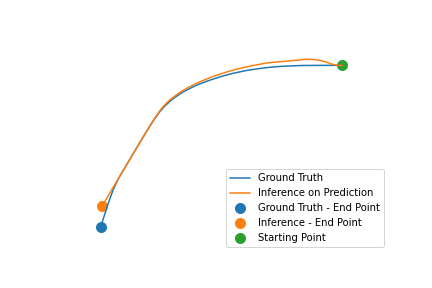
\includegraphics[width=0.48\textwidth]{images/qualitative_successful_traj1.png} \\
        % \includegraphics[width=0.48\textwidth]{images/teaser2.jpg}\\
        % \includegraphics[width=0.48\textwidth]{images/teaser3.jpg}
    \end{tabular}
    \caption{Qualitative-1}
    \label{fig:qualitative_1}
\end{figure}

\begin{figure}[h]
    \centering
    \begin{tabular}[t]{p{0.48\textwidth} }
    { \centering \small {\textit{\textbf{Command: }``Park near the tallest building.''}}}\\
        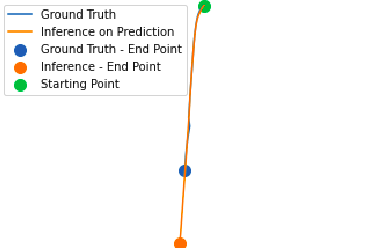
\includegraphics[width=0.48\textwidth]{images/qualitative_successful_traj22.png} \\
        % \includegraphics[width=0.48\textwidth]{images/teaser2.jpg}\\
        % \includegraphics[width=0.48\textwidth]{images/teaser3.jpg}
    \end{tabular}
    \caption{Qualitative-2}
    \label{fig:qualitative_2}
\end{figure}

\section{Real-time Navigation}

% \includemovie{1cm}{1cm}{images/full_video.gif}
% \caption{stop as soon as you encounter a white car}


The toolkit allows using the learnt model in real time, using a synchronous CARLA environment which allows capture of frames from the RGB camera and process the outputs of network to predict the next target to be shared to the simple navigation planner. A rule based approach allows us to define the intermediate target locations which is derived from the predicted segmentation masks and the predicted trajectory. Another rule based method is employed to decide if the current predicted target location is the final position for a particular command or not.

The rule for determining the target location is as follows:
\begin{itemize}
    \item Threshold the segment maps.
    \item Divide the segmentation maps into disconnected components.
    \item For the component with largest sum of probabilities, find the weighted centroid.
    \item If the sum of the values of the largest component in the final target prediction mask is higher than the threshold:
    \begin{itemize}
        \item If the sum of values of the largest component intermediate target prediction mask is higher than that of the final target prediction mask, we use the weighted centroid of that components as the intermediate target.
        \item Else, choose the weighted centroid of that component as the one of the final target predictions.
    \end{itemize}
    \item If the sum of values of the largest component in the final target prediction is less than the threshold, we use the farthest point of the trajectory prediction as the intermediate target position.
\end{itemize}

Three final predictions during a run ends the current run.

The rule for determining the target location is as follows:

\begin{algorithm}
    \caption{Target Determination}
    Target Segmentation Mask $\textbf{M}$ of dimension $(\textrm{mask\_dim} \times \textrm{mask\_dim} \times 2)$. First channel of $\textbf{M}$ responsible for first intermediate targets prediction, and second channel of $\textbf{M}$ responsible for first final targets prediction \\
    Trajectory Mask $\textbf{T}$ of dimension $(\textrm{mask\_dim} \times \textrm{mask\_dim})$
    \begin{algorithmic}[1]
        \Procedure{PredictNextTarget}{$\textbf{M}, \textbf{T}$}
            \State $\textbf{M}' \gets$ \Call{BinaryThresholding}{$\textbf{M}$}
            \State $\textbf{T}' \gets$ \Call{Skeletonize}{$\textbf{T}$}
            \State $\textbf{C}_0 \gets$ \Call{Components}{$\textbf{M}'[:,:,0]$}
            \State $\textbf{C}_1 \gets$ \Call{Components}{$\textbf{M}'[:,:,1]$}
            \If {$\sum{p}_{ p \in \max \textbf{C}_0} > \delta$}
                \If {$\sum{q}_{ q \in \max \textbf{C}_1} > \sum{p}_{ p \in \max \textbf{C}_0}$}
                    \State $\textrm{target.location} \gets$ \Call{WeightedCentroid}{$\max \textbf{C}_1$}
                    \State $\textrm{target.isFinal} \gets \textrm{False}$
                \Else
                    \State $\textrm{target.location} \gets$ \Call{WeightedCentroid}{$\max \textbf{C}_0$}
                    \State $\textrm{target.isFinal} \gets \textrm{True}$
                \EndIf
                \Else
                    \State $\textrm{target.location} \gets \Call{FarthestPoint}{\textbf{T}'}$
                    \State $\textrm{target.isFinal} \gets \textrm{False}$
            \EndIf
        \EndProcedure
    \end{algorithmic}
\end{algorithm}

\section{Conclusion}

\bibliographystyle{ieeetr}
\bibliography{iros_references}

\end{document}
